\clearpage
\section{Clustered Objects}
\label{sect:ClusteredObjects}

\subsection{Mass Fractal}
\label{sect:MassFractal}
\hspace{1pt} \\

\begin{figure}[htb]
\begin{center}
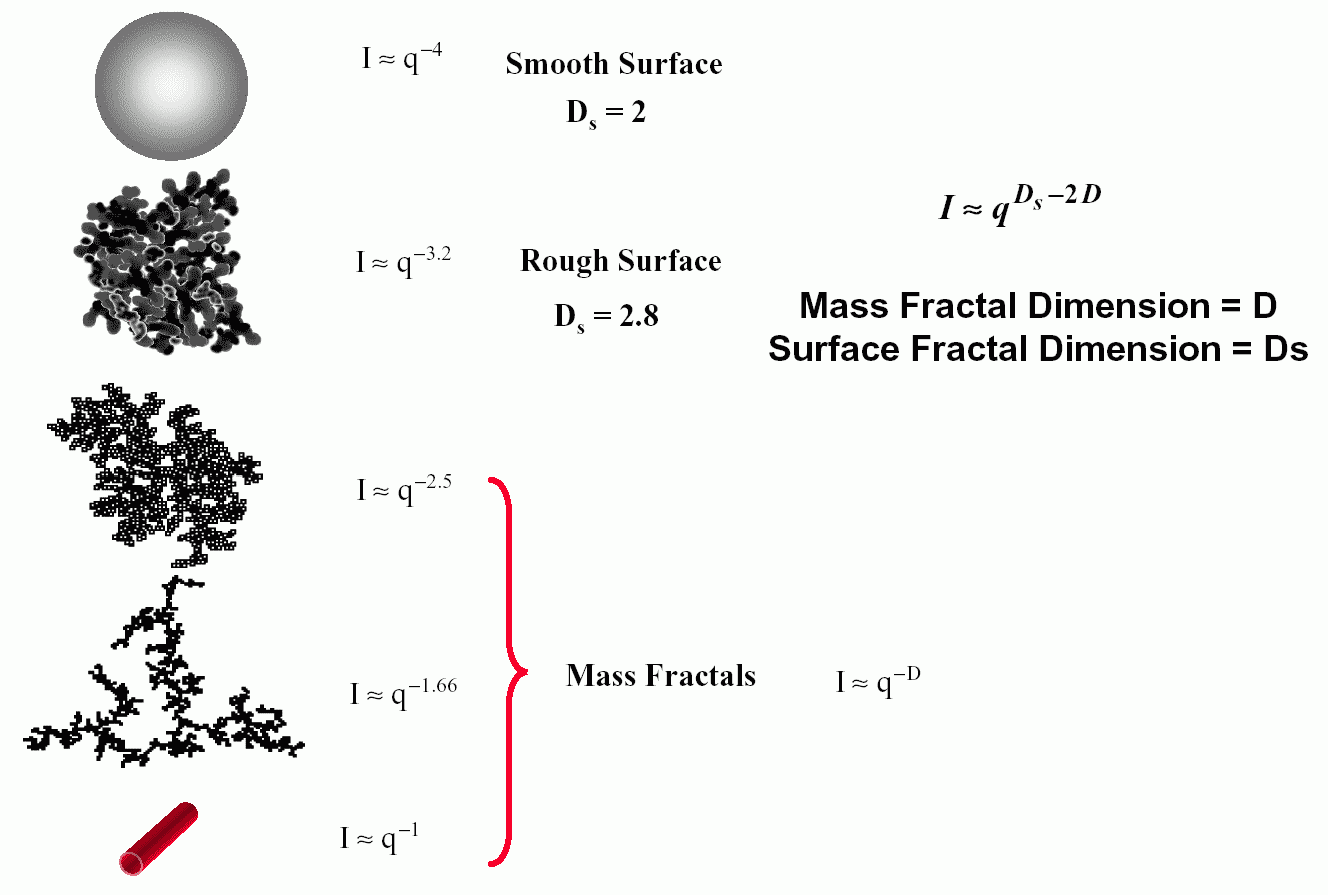
\includegraphics[width=0.9\textwidth]{../images/form_factor/cluster/fractaldimension.png}
\end{center}
\caption{} \label{fractaldimension}
\end{figure}

Aggregates and clusters often have a fractal morphology \cite{Sorensen1999,Sorensen1992,Hurd1988,Lin1989,Lin1990,Lin1990a,Lin1990b}. These self-similar clusters are well
described by
\begin{align}
N=k_0(R_g/r_0)^D
\end{align}
where $N$ is the number of primary particles or monomers in the aggregate,
$k_0$ is a constant of order unity, $R_g$ is the radius of gyration of the aggregate,
$r_0$ is the monomer radius, and $D$ is the fractal dimension.

The scattering function and the density autocorrelation function
of the aggregate are Fourier transform pairs; thus
\begin{align}
I(q)=4\pi \int_0^\infty \, g(r)\, r^2\, \frac{\sin(qr)}{qr}\, dr
\label{eq:aggregateSQ}
\end{align}
For a fractal aggregate the autocorrelation function has the
form
\begin{align}
g(r) \sim r^{D-d} h(r,\xi)
\label{eq:aggregate_g(r)}
\end{align}
Here $D$ is the fractal dimension, $d$ the spatial dimension, and
$\xi$ a measure of the linear size of the aggregate proportional to
the radius of gyration $R_g$. The function $h(r,\xi)$ is the cutoff
function describing the perimeter of the aggregate. Its properties
are that $h(r,\xi) \simeq 1$ for $r/\xi \lesssim 1$, but for large
$r/\xi$ it falls off faster than any power law.

\noindent

\begin{table}[htb]
\caption{Scattering functions $I(q)$ for different cutoff functions
$h(r,\xi)$.
\label{tab:SQ_cutuofffunctions}}
\begin{tabular}{|c|c|c|c|c|}
  \hline
  & & & & \\[-2mm]
  % after \\: \hline or \cline{col1-col2} \cline{col3-col4} ...
  {\tt SASfit}-name & $h(r,\xi)$    & $\xi^2$   & $I(q)$    & Ref. \\
  & & & & \\[-2mm]
  \hline
  \hline
  & & & & \\[-2mm]
   {\tt \scriptsize Fisher-Burford}&  $\scriptstyle \text{ca. } \exp\left[-\tfrac{r}{\xi}\right]$  & $\scriptstyle R_g^2/3$ & $\scriptstyle \left(1+\frac{2}{3D}q^2R_g^2\right)^{-D/2}$ &  \cite{Fisher1967}\\[3mm]
   {\tt \scriptsize MassFractExp}   & $\scriptstyle \exp\left[-\tfrac{r}{\xi}\right]$          & $\frac{2R_g^2}{D(D+1)}$ & $\scriptstyle \frac{\sin\left[(D-1)\arctan(q\xi)\right]}{(D-1)q\xi(1+q^2\xi^2)^{(D-1)/2}}$ &  \cite{Sorensen1999}\\[3mm]
   {\tt \scriptsize MassFractGauss} & $\scriptstyle \exp\left[-\left(\tfrac{r}{\xi}\right)^2\right]$ & $\frac{4R_g^2}{D}$ & $\scriptstyle e^{-\frac{q^2R_g^2}{D}} {}_1F_1\left[\frac{3-D}{2},\frac{3}{2},\frac{q^2R_g^2}{D}\right]$ &  \cite{Sorensen1992}\\[3mm]
   $\text{\tt \scriptsize Aggregate}\atop \text{\tt (Exp(-x$\hat~$a) Cut-Off)}$ & $\scriptstyle \exp\left[-\left(\tfrac{r}{\xi}\right)^\alpha\right]$ & --- & numerical &  \cite{Sorensen2001}\\[3mm]
   $\text{\tt \scriptsize Aggregate}\atop \text{\tt (OverlapSph Cut-Off)}$ & $ \scriptstyle
                                                    \begin{cases}\scriptstyle
                                                        \left(1+\tfrac{r}{4\xi}\right) \left(1-\tfrac{r}{2\xi}\right)^2 ,&  \scriptstyle r<2\xi\\
                                                        \scriptstyle 0 ,&  \scriptstyle r\geq 2\xi
                                                  \end{cases}$ & $\scriptstyle\frac{(D+2)(D+5)}{2D(D+1)}R_g^2$ & numerical &  \cite{Hurd1988}\\[3mm]
   {\tt \scriptsize DLCAggregate} & --- & --- & $\scriptstyle \left[1+{\displaystyle \sum_{\scriptstyle s=1}^{\scriptstyle 4}}C_s(qR_g)^{2s}\right]^{-D/8}$ &  \cite{Lin1990c}\\
                                          & & & $\scriptstyle C_1=\frac{8}{3D}, \, C_2=2.5$ & \\
                                          & & & $\scriptstyle C_3=-1.52, \, C_4=1.02$ & \\[3mm]
   {\tt \scriptsize RLCAggregate} & --- & --- & $\scriptstyle C_1=\frac{8}{3D}, \, C_2=3.13$ & \\
                                          & & & $\scriptstyle C_3=-2.58, \, C_4=0.95$ & \cite{Lin1990c}\\[3mm]
  \hline
\end{tabular}
\end{table}


\begin{figure}[htb]
\begin{center}
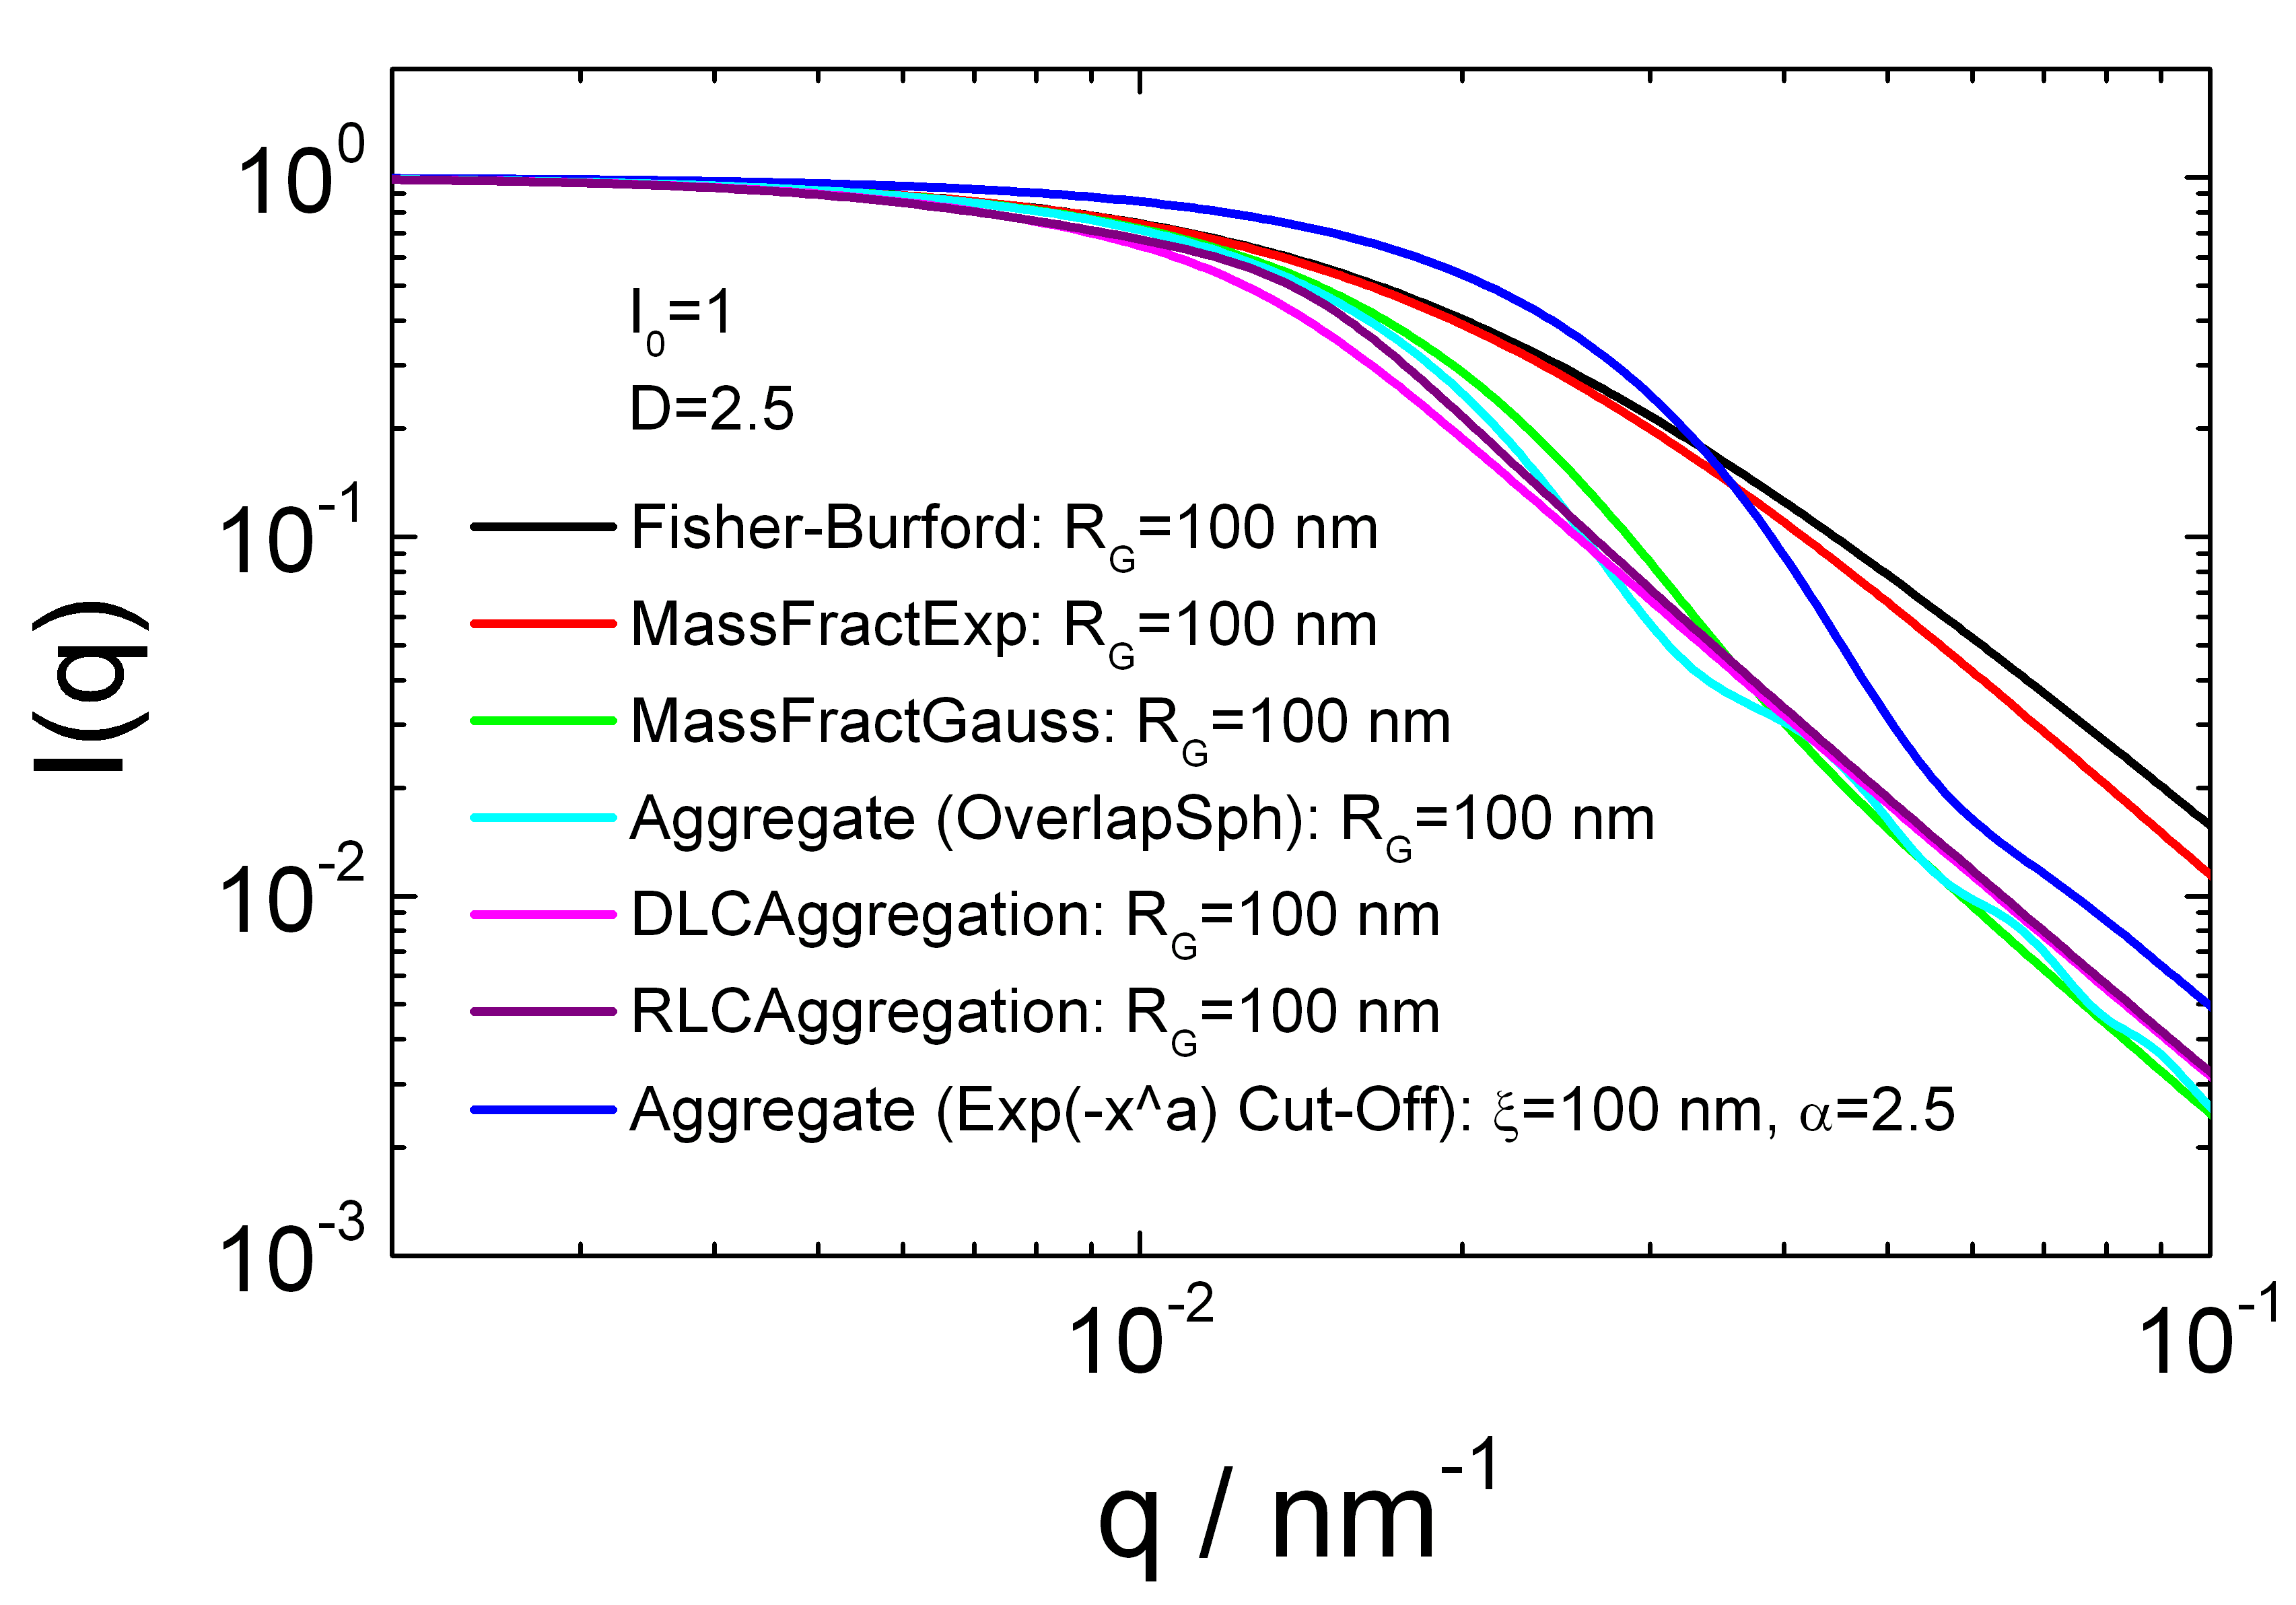
\includegraphics[width=0.768\textwidth]{../images/form_factor/cluster/AggregateComparison.png}
\end{center}
\caption{Form factor for the different types of mass fractals listed in \ref{tab:SQ_cutuofffunctions}.}
\label{fig:FFCluster}
\end{figure}

%%%%%%%%%%%%%%%%%%%%%%%%%%%%%%%%%%%%%%%%%%%%%%%%%%%%%%%%%%%%%%%%%%


\clearpage
\subsection{Stacked Discs}
\label{sect:StackedDiscs}
~\\

\begin{figure}[htb]
\begin{center}
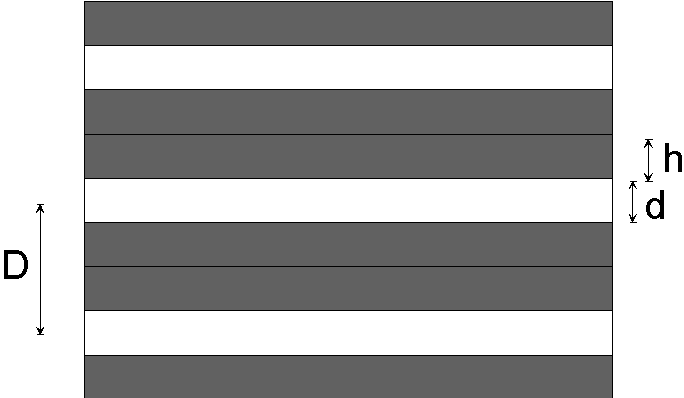
\includegraphics[width=0.5\textwidth]{../images/form_factor/cluster/stackdiscs.png}
\end{center}
\caption{Sketch for a stack of discs with an additional surface layer}
\label{stackeddiscs}
\end{figure}



\begin{align}
I_\text{StackedDiscs}(Q,R)&= \int_0^{\pi/2}\left( \Delta\eta_l
\left(V_t f_t - V_c f_c\right) + \Delta\eta_c  V_c f_c \right)^2
S(Q,\Theta) \sin(\Theta)\, d\Theta
\end{align}
Here \cite{Kratky1949,Frielinghaus2017,Vaia2002,Hanley2003} it is assume that the nearest neighbor distance between the
platelets obeys a Gaussian distribution and consider an internal
structure factor, $S(Q,\Theta)$, first proposed by Kratky and Porod
in 1949 \cite{Kratky1949}
\begin{align}
S(Q,\Theta) &=  1+\frac{2}{n} \sum_{k=1}^{n-1} (n-k)
\cos(kDQ\cos(\Theta))
     \exp\left(-\frac{k}{2}\left(Q\cos(\Theta) \sigma_D\right)^2\right) \\
f_t &= f_t = \frac{\sin\left(Q(\frac{d}{2}+h)\cos(\Theta)\right)}{Q(\frac{d}{2}+h)\cos(\Theta)} \,\,\,\,2\frac{J_1(QR\sin(\Theta))}{QR\sin(\Theta)} \\
f_c &= f_c = \frac{\sin\left(Q\frac{d}{2}\cos(\Theta)\right)}{Q\frac{d}{2}\cos(\Theta)} \,\,\,\,2\frac{J_1(QR\sin(\Theta))}{QR\sin(\Theta)}\\
V_t &= \pi R^2 (d+2h)\\
V_c &= \pi R^2 d
\end{align}


\begin{figure}[htb]
\begin{center}
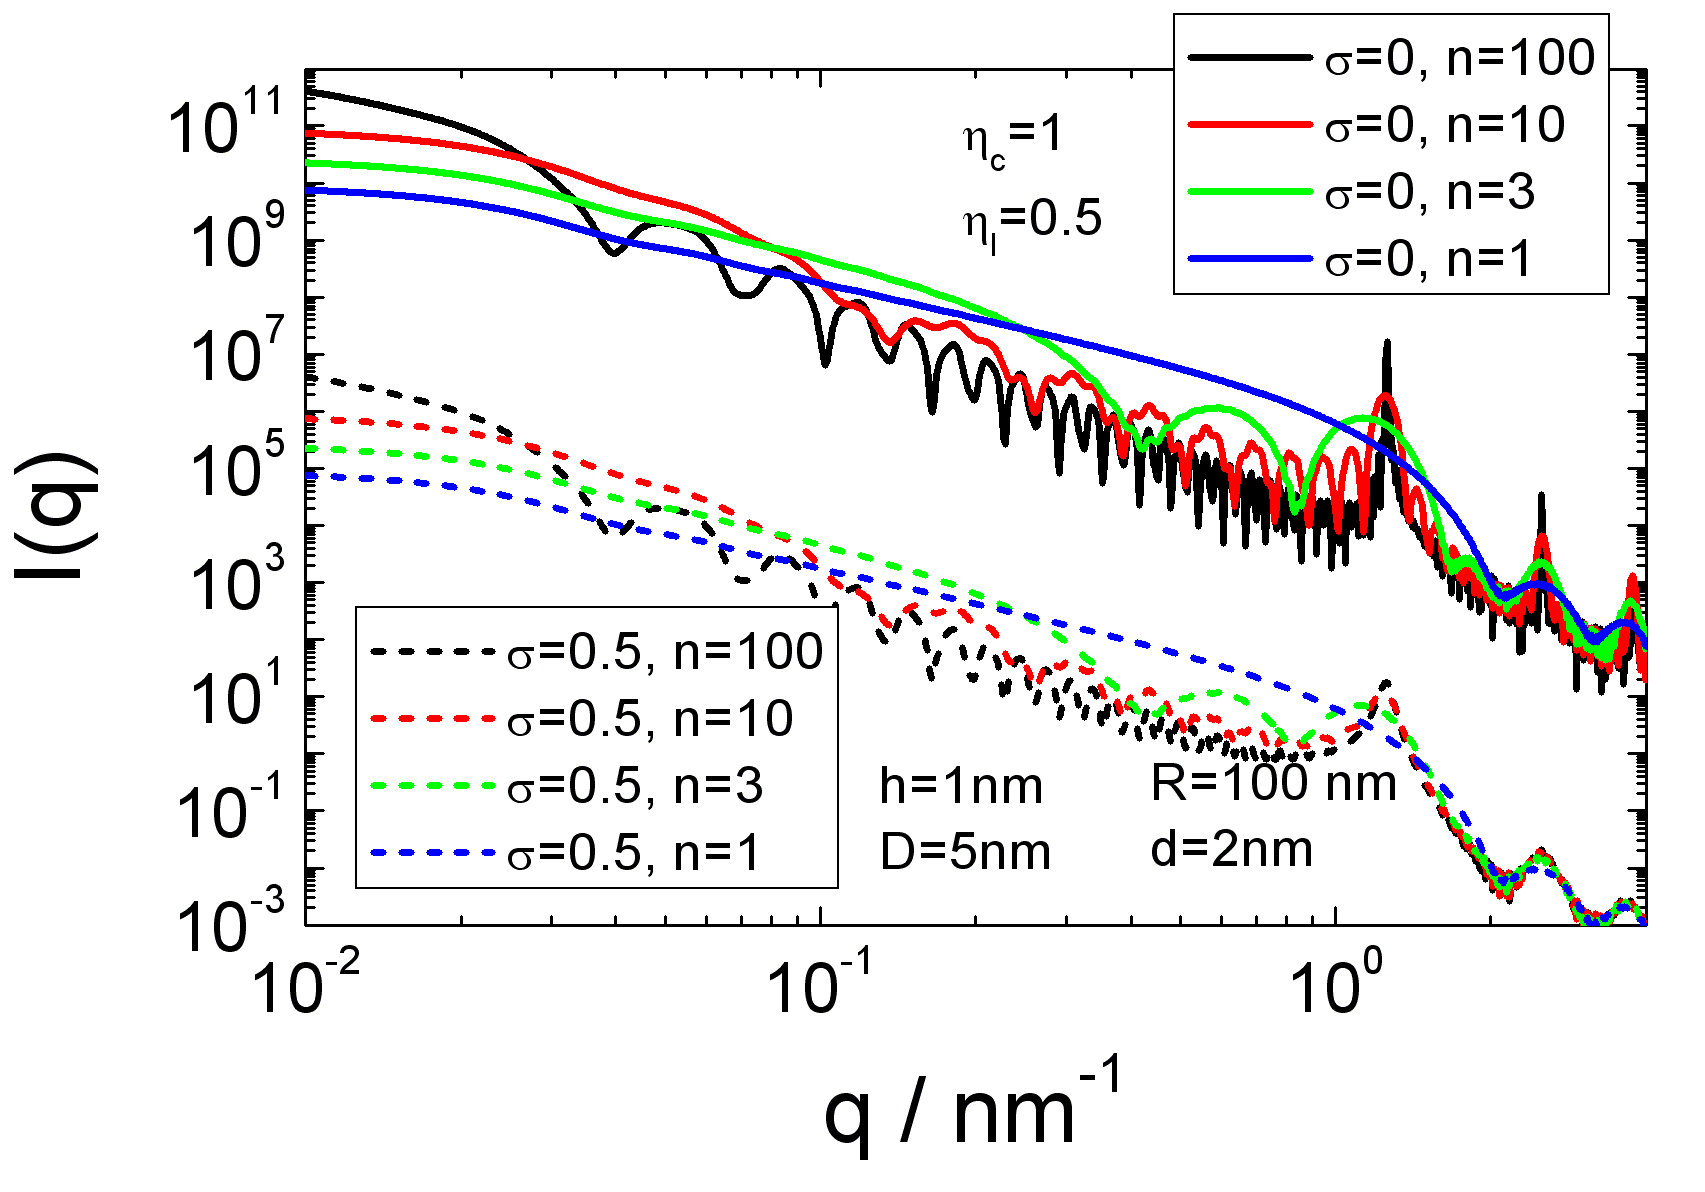
\includegraphics[width=0.768\textwidth]{../images/form_factor/cluster/StackedDiscsIQ.png}
\end{center}
\caption{Scattering Intensity for a stack of discs with a layer.}
\label{fig:StackedDiscs}
\end{figure}

%%%%%%%%%%%%%%%%%%%%%%%%%%%%%%%%%%%%%%%%%%%%%%%%%%%%%%%%%%%%%%%%%%%%%%

\clearpage
\subsection{DumbbellShell}
\label{sect:DumbbellShell}
~\\

\begin{figure}[htb]
\begin{center}
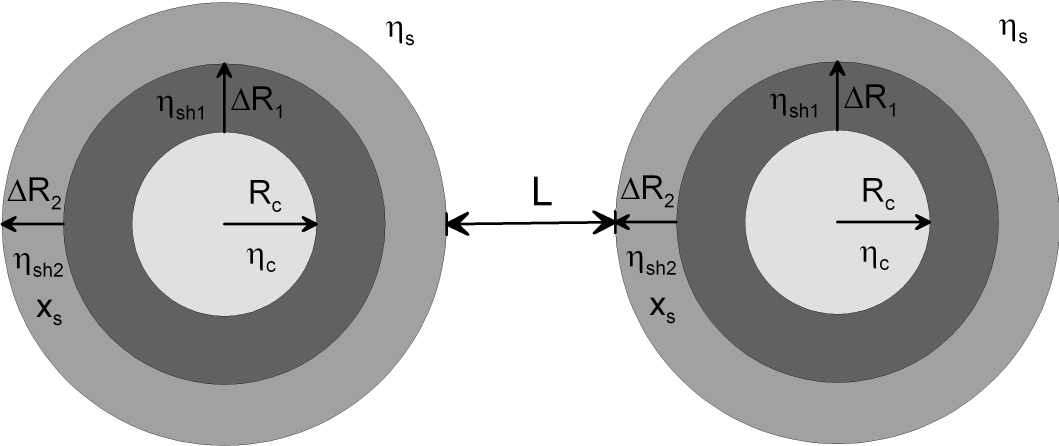
\includegraphics[width=0.8\textwidth]{../images/form_factor/cluster/l_doubleshell.png}
%1059x446
\end{center}
\caption{} \label{DumbbellShell}
\end{figure}

%%%%%%%%%%%%%%%%%%%%%%%%%%%%%%%%%%%%%%%%%%%%%%%%%%%%%%%%%%%%%%%%%%%%%%%%%%%%%%%%%%%%%%

\clearpage
\subsection{DoubleShellChain}
\label{sect:DoubleShellChain}
~\\

\begin{figure}[htb]
\begin{center}
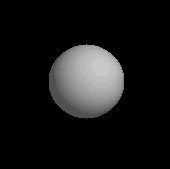
\includegraphics[width=0.18\textwidth]{../images/form_factor/cluster/tetrahedron1.png}
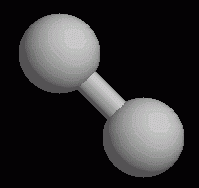
\includegraphics[width=0.18\textwidth]{../images/form_factor/cluster/tetrahedron2.png}
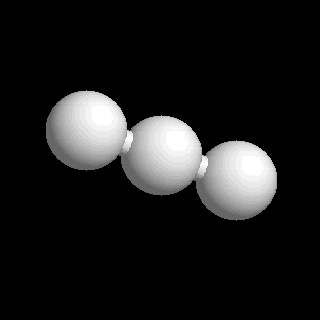
\includegraphics[width=0.18\textwidth]{../images/form_factor/cluster/DoubleShellChain3.png}
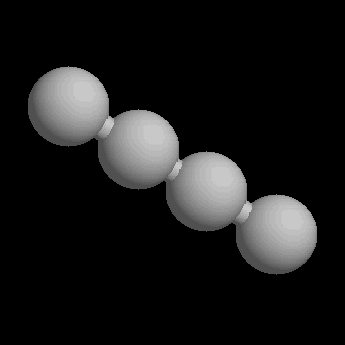
\includegraphics[width=0.18\textwidth]{../images/form_factor/cluster/DoubleShellChain4.png}
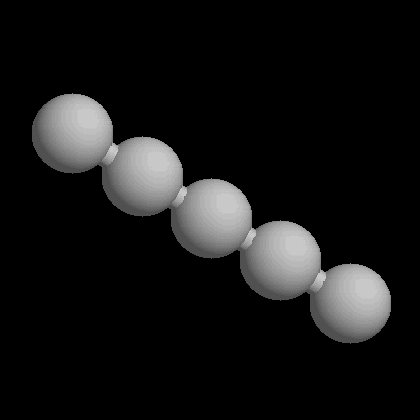
\includegraphics[width=0.18\textwidth]{../images/form_factor/cluster/DoubleShellChain5.png}
\end{center}
\caption{} \label{doubleshellchain}
\end{figure}

\begin{figure}[htb]
\begin{center}
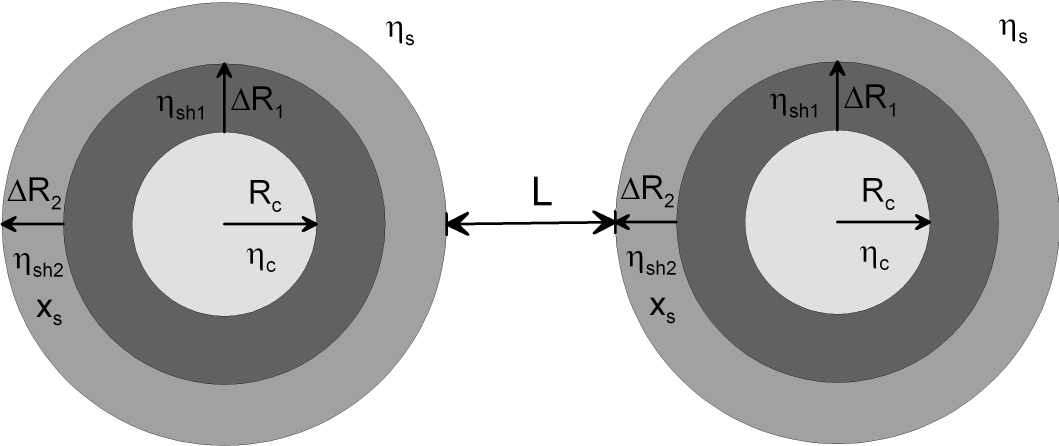
\includegraphics[width=0.8\textwidth]{../images/form_factor/cluster/l_doubleshell.png}
%1059x446
\end{center}
\caption{} \label{doubleshell}
\end{figure}

\begin{figure}[htb]
\begin{center}
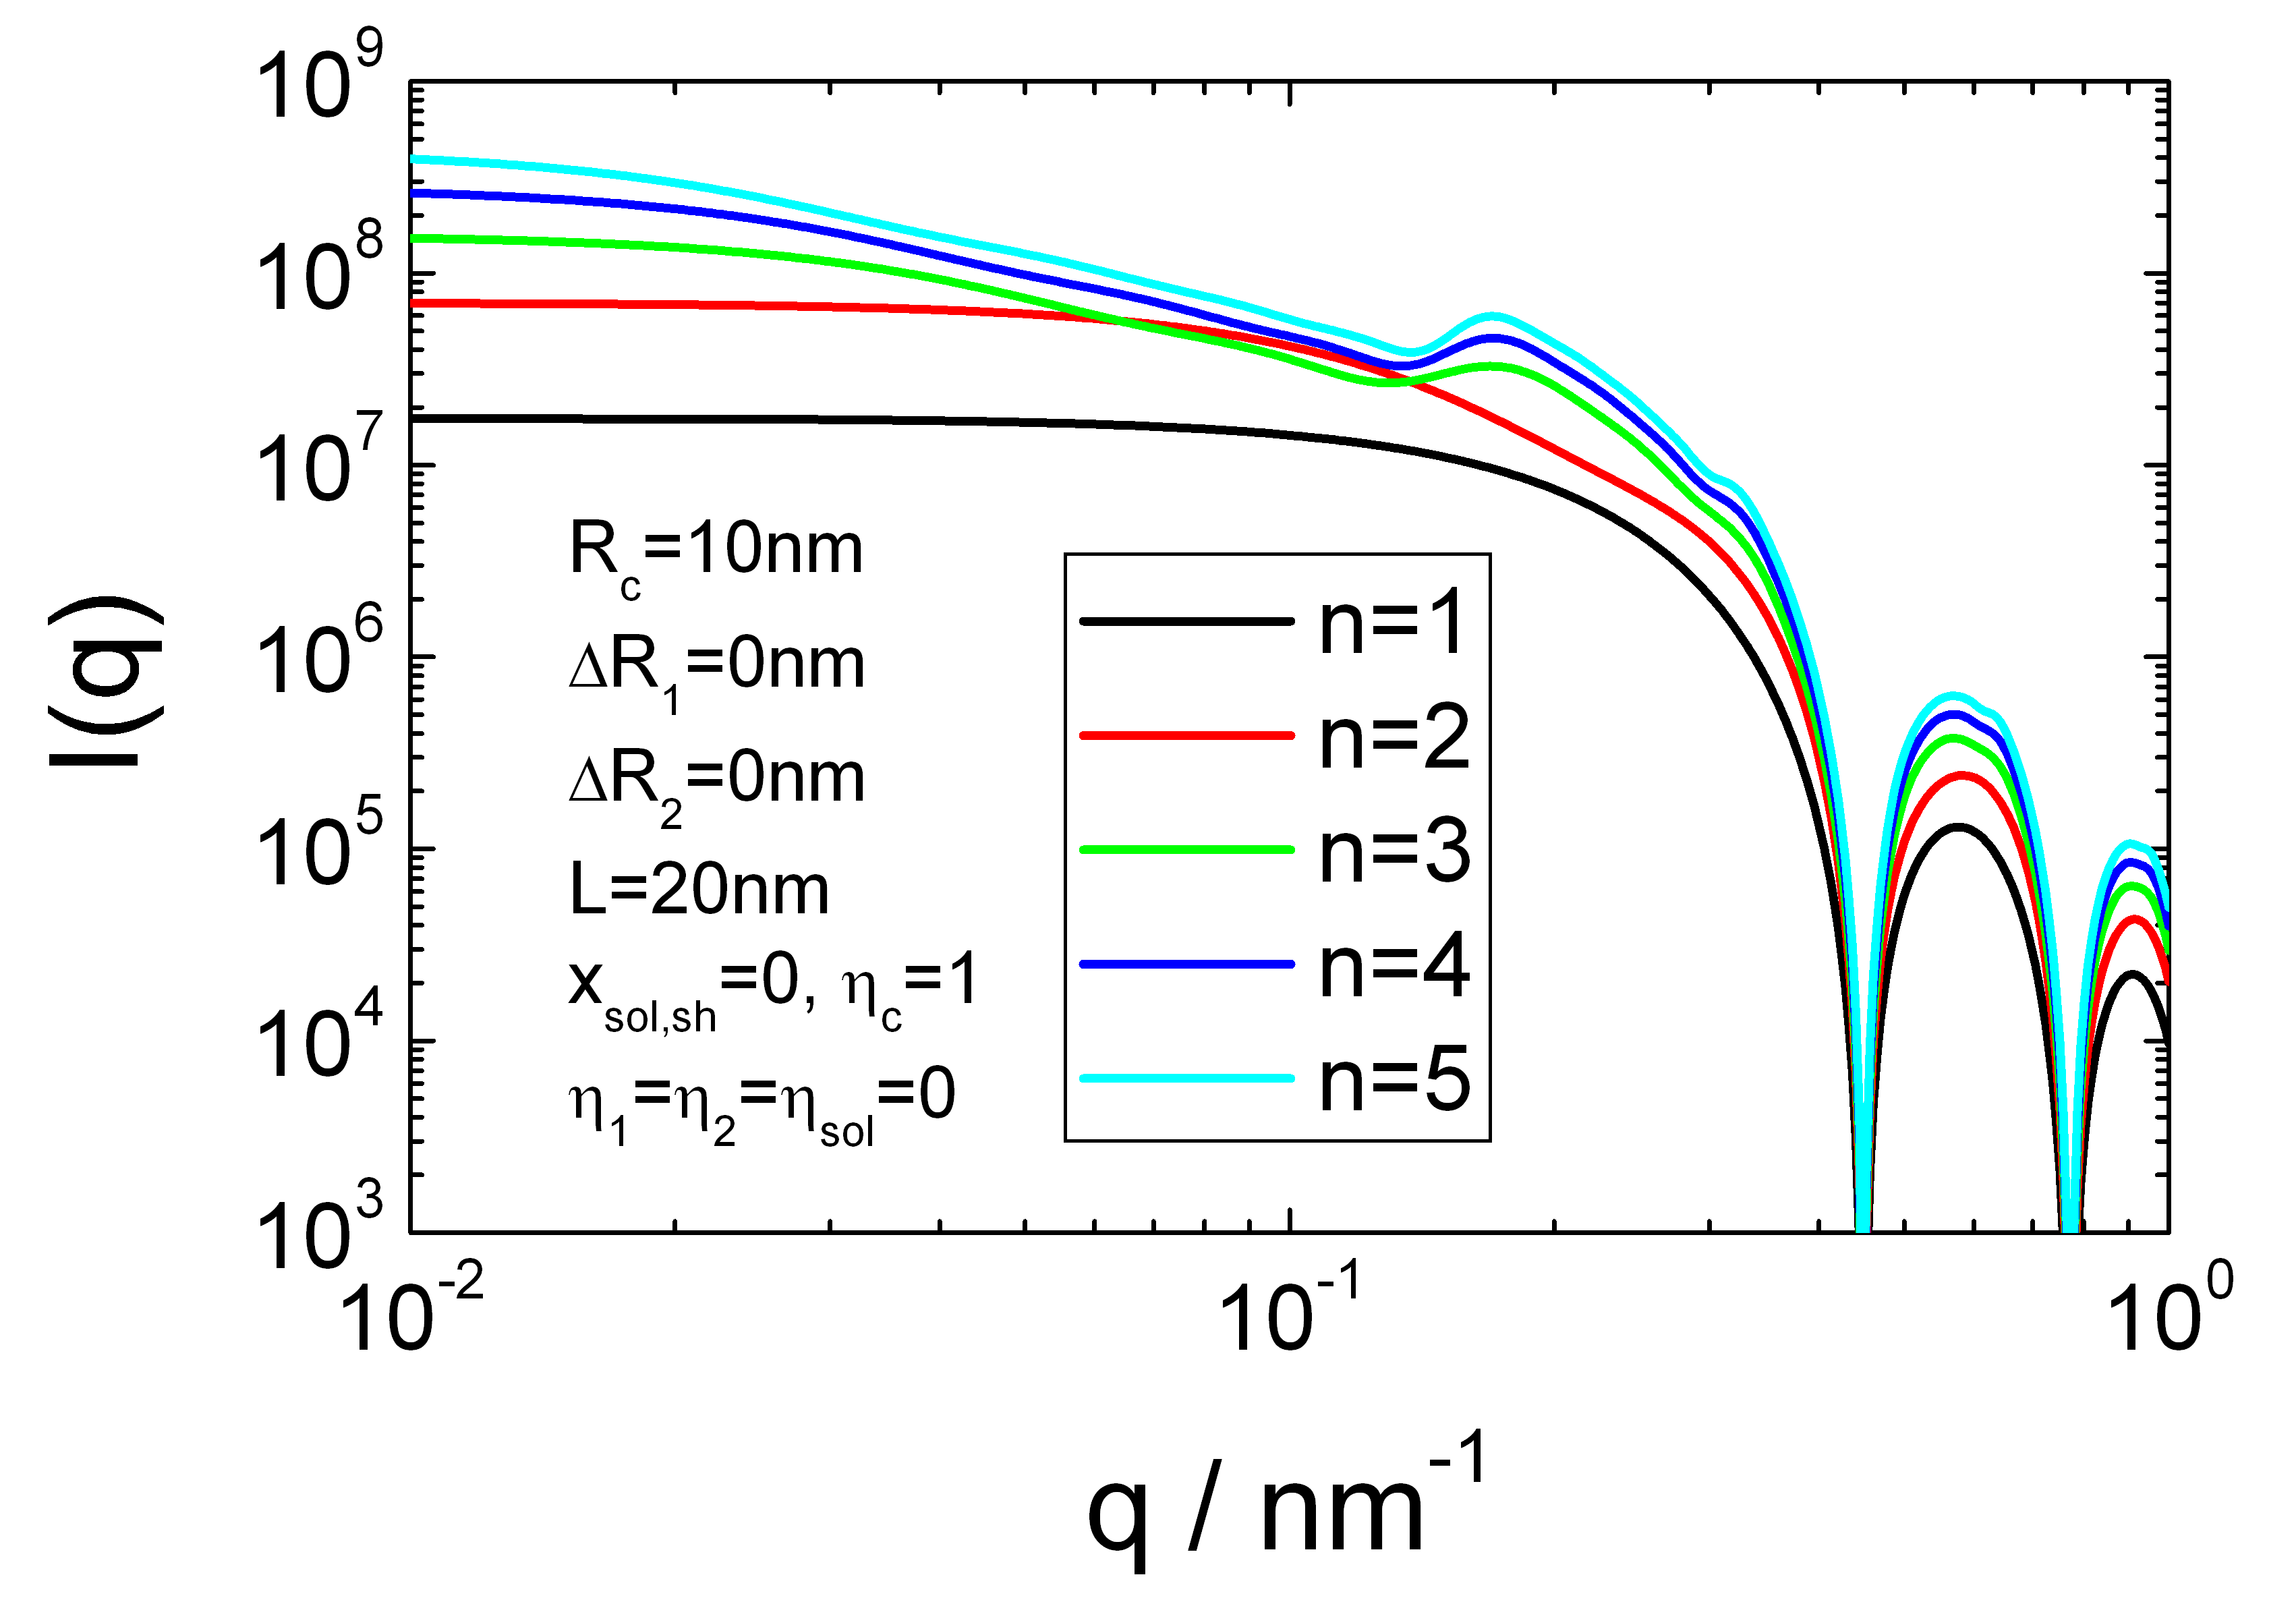
\includegraphics[width=0.8\textwidth]{../images/form_factor/cluster/DoubleShellChain.png}
\end{center}
\caption{}
\label{fig:DoubleShellChain}
\end{figure}

%%%%%%%%%%%%%%%%%%%%%%%%%%%%%%%%%%%%%%%%%%%%%%%%%%%%%%%%%%%%%%%%%%%%%%%%%%%%%%



\begin{figure}[htb]
\begin{center}
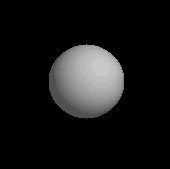
\includegraphics[width=0.18\textwidth]{../images/form_factor/cluster/tetrahedron1.png}
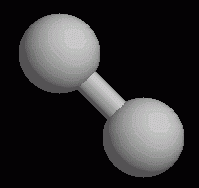
\includegraphics[width=0.18\textwidth]{../images/form_factor/cluster/tetrahedron2.png}
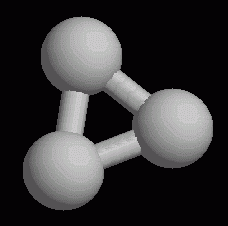
\includegraphics[width=0.18\textwidth]{../images/form_factor/cluster/tetrahedron3.png}
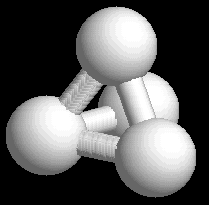
\includegraphics[width=0.18\textwidth]{../images/form_factor/cluster/tetrahedron4.png}
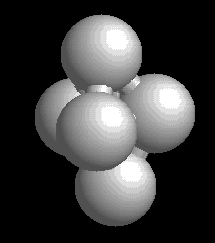
\includegraphics[width=0.18\textwidth]{../images/form_factor/cluster/tetrahedron5.png}
\end{center}
\caption{} \label{tetrahedron}
\end{figure}
\begin{figure}[htb]
\begin{center}
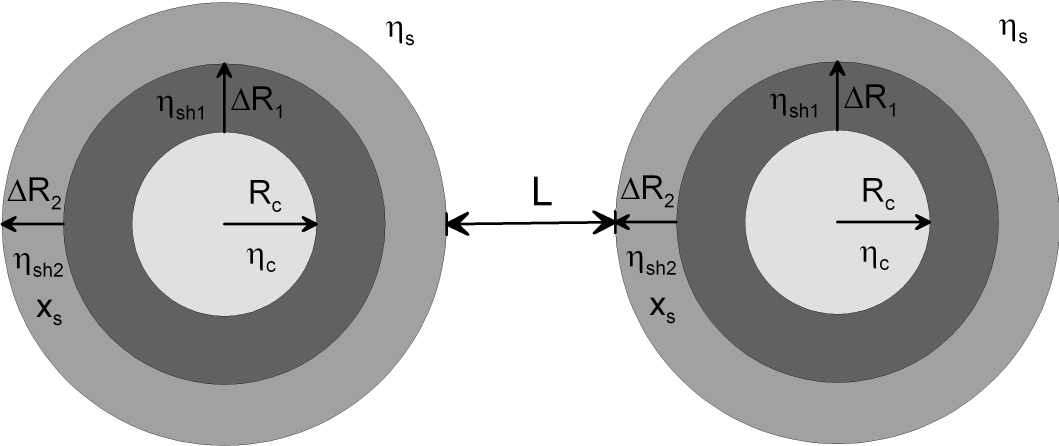
\includegraphics[width=0.8\textwidth]{../images/form_factor/cluster/l_doubleshell.png}
%1059x446
\end{center}
\caption{}
\label{TetrahedronDoubleShell}
\end{figure}

\begin{figure}[htb]
\begin{center}
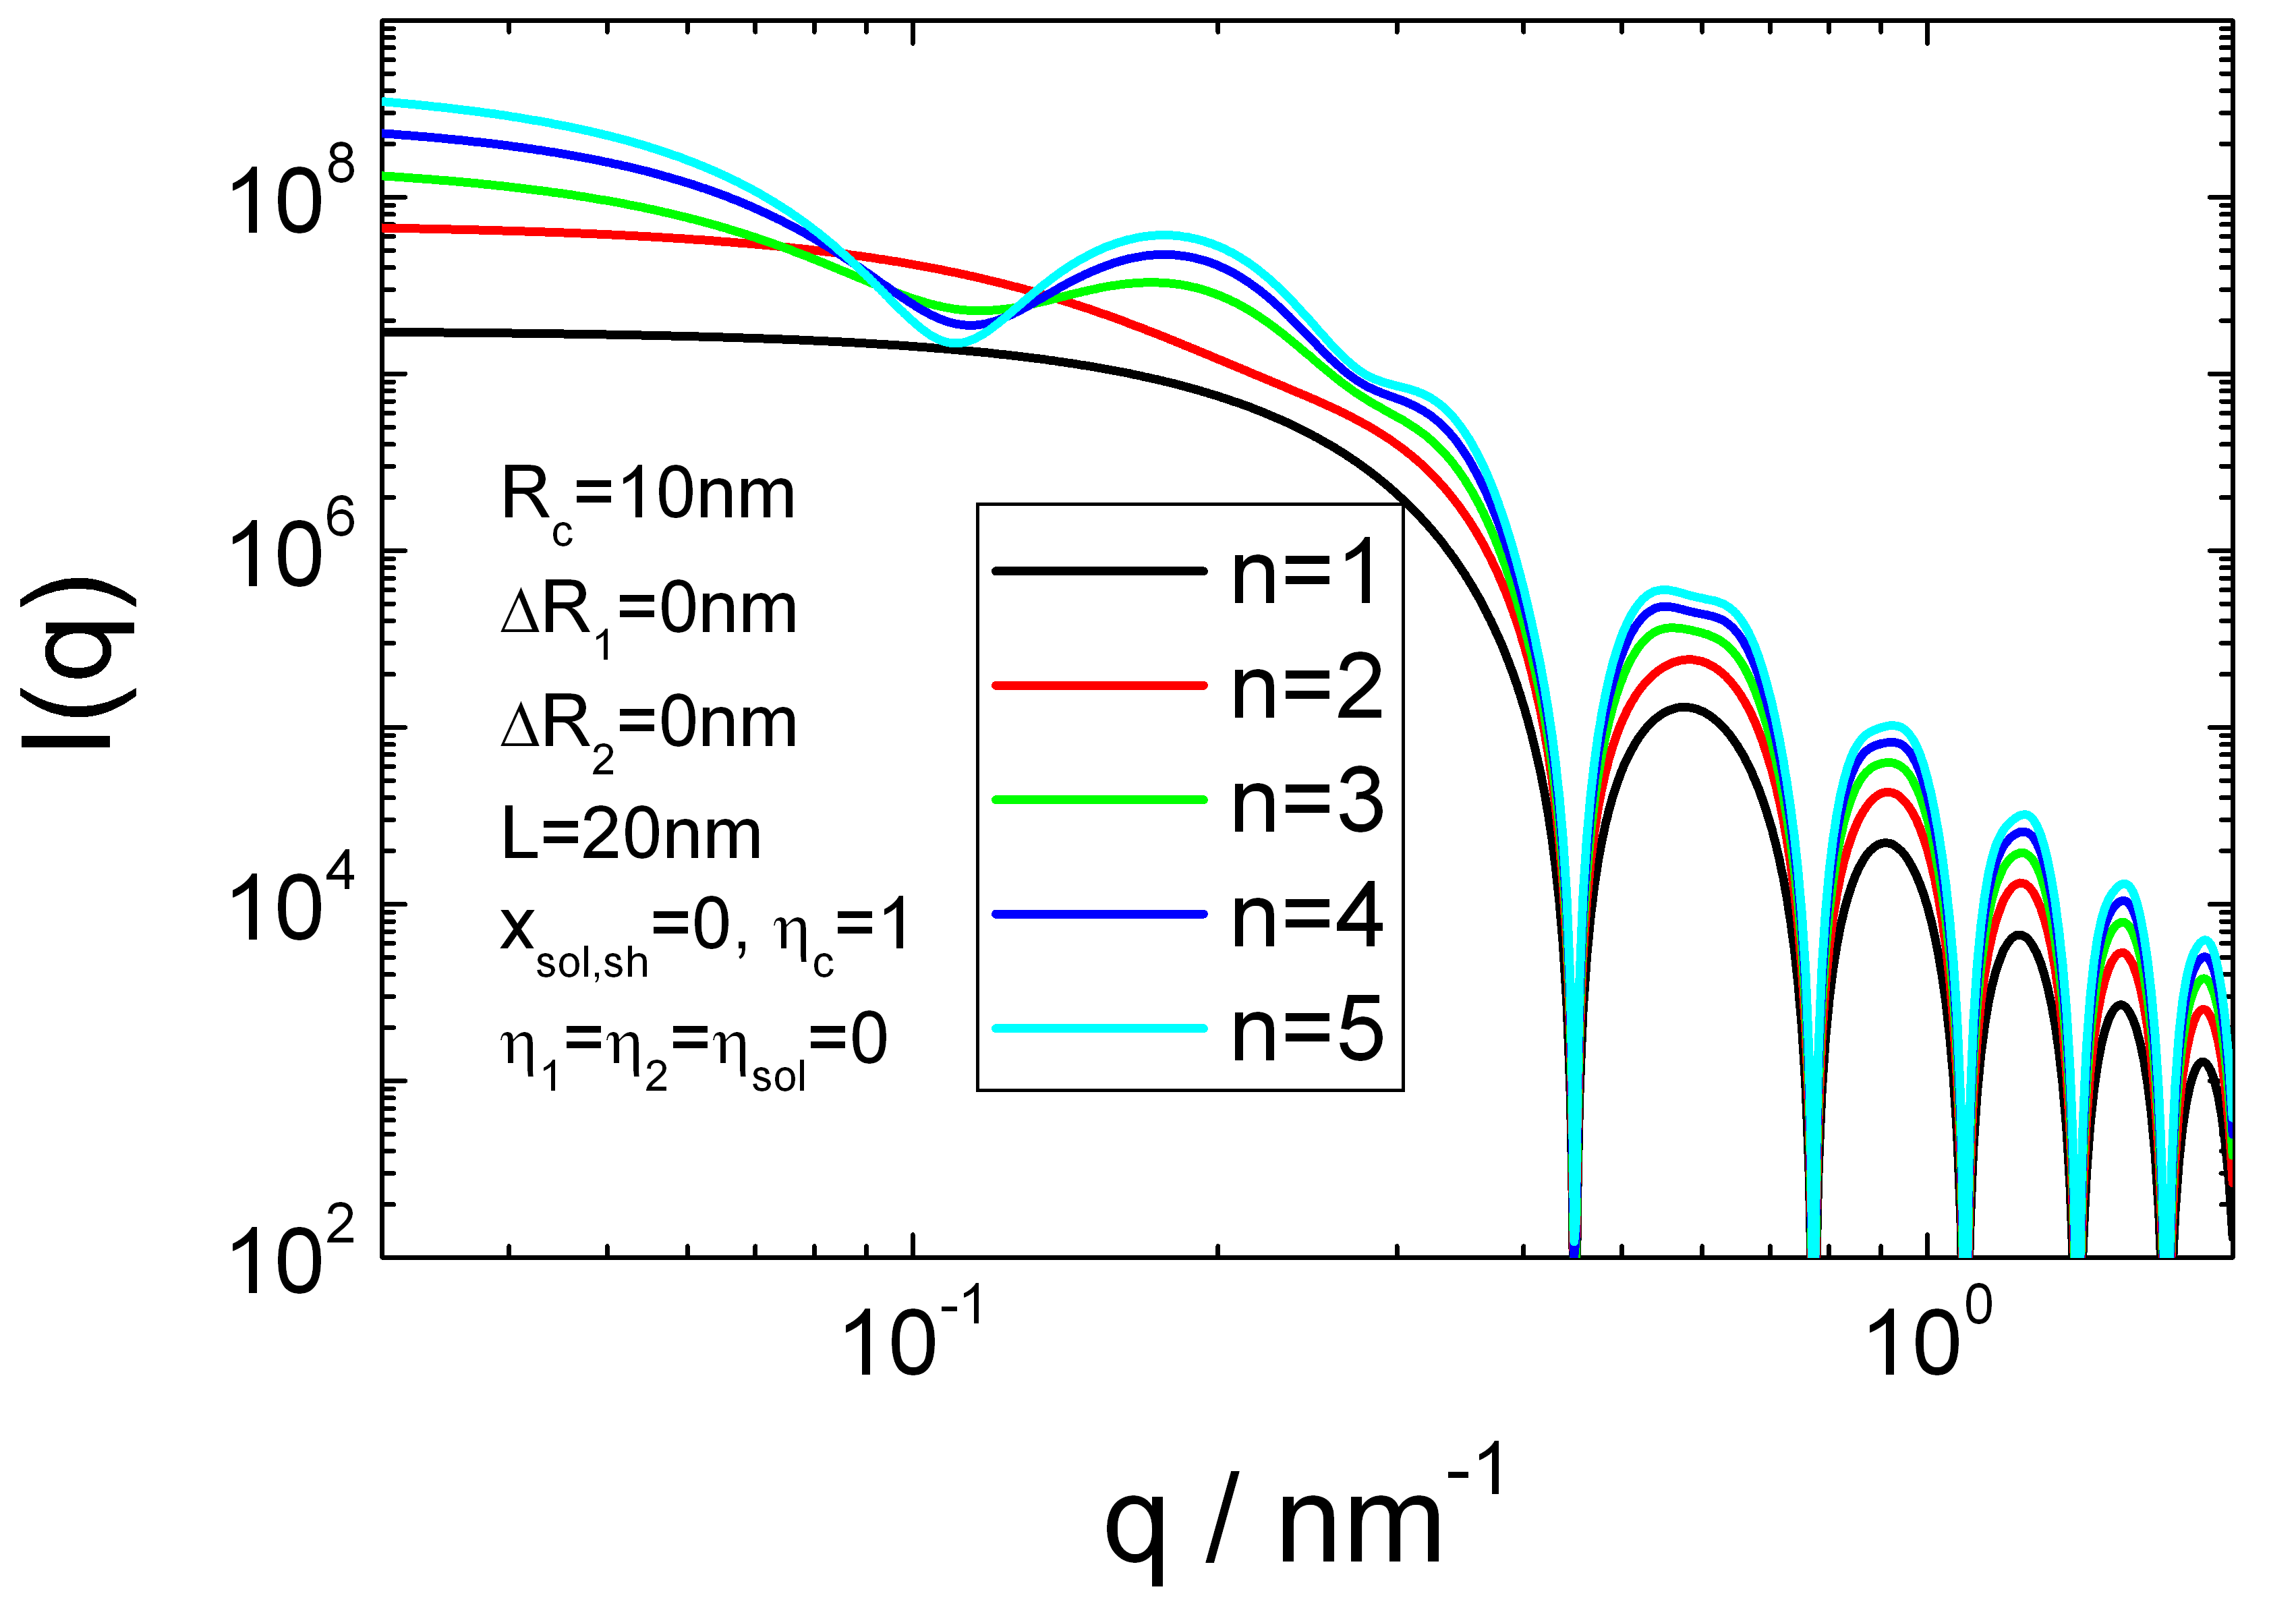
\includegraphics[width=0.8\textwidth]{../images/form_factor/cluster/TetraHedronDoubleShell.png}
\end{center}
\caption{}
\label{fig:TetrahedronDoubleShell}
\end{figure}


%%%%%%%%%%%%%%%%%%%%%%%%%%%%%%%%%%%%%%%%%%%%%%%%%%%%%%%%%%%%%%%%%%%%%%%%%%%%%%%%%%%%%%%%
\clearpage
\subsection{fractal size distribution of particles} \hspace{1pt}
\label{sec:ff_fractal_series}

Scattering curves of samples having a fractal structure show on a log–log scale a linear behaviour.
One way to define the fractal dimension of an object is to look how the mass $m$ of an object scales
with its size $x$. For an object with a fractal dimension of $f_D$ the mass scales $m$
with $m \propto x^{f_D}$. A similar behaviour also can be found if the sample contains
particles with a size distribution $n(x)$ proportional to $\propto x^{-(1+f_D)}$.
\begin{align}
n(x,N,f_D,x_\mathrm{min},x_\mathrm{max}) &=
\begin{cases}
x < x_\mathrm{min} & 0 \\
x_\mathrm{min}\leq x \leq x_\mathrm{max} & N \frac{x^{-(1+f_D)}}{\left(x_\mathrm{min}^{-f_D}-x_\mathrm{max}^{-f_D}\right)/f_D} \\
x > x_\mathrm{max}  & 0
\end{cases}
\end{align}
The integral over size distribution $\int n(x,N,f_D,x_\mathrm{min},x_\mathrm{max}) \mathrm{d}x$ is normalized to $N$.
In case the distribution follows such a potential law over a large enough size range a slope of
$Q^{-(6-f_D)}$ in the scattering curve will be observed similar to the scattering behaviour
of a surface fractal. Deviations of it can occur if the size range $[x_\mathrm{min},x_\mathrm{max}]$
of such a size distribution is to narrow. The integration of a spherical form factor
$
I(Q) = \int_{\xi_\mathrm{min}}^{\xi_\mathrm{max}} N\frac{r^{-(1+f_D)}}{\left(R_\mathrm{min}^{-f_D}-R_\mathrm{max}^{-f_D}\right)/f_D} \left(\frac{4}{3}\pi r^3 \frac{\sin Qr - Qr \cos Qr}{(Qr)^3}\right)^2 \mathrm{d}r
$
has not been found yet. However, using the Debye-Anderson-Brumberger (DAB) model from \ref{sect:DAB}
instead of the form factor for spheres allows to express the integral in terms of hypergeometric functions:
\begin{flalign}
I_{f_D}(Q;N,f_D,\xi_\mathrm{min},\xi_\mathrm{max}) &= \int_0^\infty n(\xi,N,f_D,\xi_\mathrm{min},\xi_\mathrm{max})  \xi^6 I_\text{DAB}(Q,\xi) \mathrm{d}\xi\\
&= \int_{\xi_\mathrm{min}}^{\xi_\mathrm{max}} N\frac{\xi^{-(1+f_D)}}{\left(\xi_\mathrm{min}^{-f_D}-\xi_\mathrm{max}^{-f_D}\right)/f_D}   \frac{\xi^6}{\left(1+\xi^2Q^2\right)^2}
 \mathrm{d}\xi \\
&= N\frac{({f_D}-4){f_D}}{\left({f_D}-2\right) 2 Q^4
   \left(\xi_\mathrm{max}^{{f_D}}-\xi_\mathrm{min}^{{f_D}}\right)}
    \Bigg[  \nonumber \\
\begin{split}
    \xi_\mathrm{max}^2 \xi_\mathrm{min}^{{f_D}} \,
   _2F_1\left(1,\frac{{f_D}-2}{2};\frac{{f_D}}{2};-\frac{1}{Q^2 \xi_\mathrm{max}^2}\right) \\
    -\xi_\mathrm{min}^2 \xi_\mathrm{max}^{{f_D}} \,
   _2F_1\left(1,\frac{{f_D}-2}{2};\frac{{f_D}}{2};-\frac{1}{Q^2
   \xi_\mathrm{min}^2}\right)\Bigg]
\end{split} \\
&+
   N\frac{
   {f_D} Q^2 \left(\frac{\xi_\mathrm{min}^4
   \xi_\mathrm{max}^{{f_D}}}{Q^2 \xi_\mathrm{min}^2+1}-\frac{\xi_\mathrm{max}^4
   \xi_\mathrm{min}^{{f_D}}}{Q^2 \xi_\mathrm{max}^2+1}\right)}{2 Q^4
   \left(\xi_\mathrm{max}^{{f_D}}-\xi_\mathrm{min}^{{f_D}}\right)} \nonumber
\end{flalign}
The DAB Model follows a Guinier law at small $Q$-values and the Porod law $(Q^{-4})$ at large $Q$ values like a sphere. The term $\xi^6$ is added to account for the fact, that intensities scale with the squared volume of a particle. The correlation length $\xi$ in the DAB model is related to the radius of gyration $R_G$ or the radius of a sphere $R$  via $\xi^2=\frac{1}{6} R_G^2=\frac{5}{18} R^2$.\footnote{
The Taylor series of the DAB model at small Q-values gives $I_\text{DAB}(Q\rightarrow 0,\xi) \sim 1-2\xi^2Q^2+3\xi^4Q^4$ whereas the Taylor series of a form factor in terms of the Guinier radius $R_G$ or the Guinier law at small Q-values is $I(Q\rightarrow 0)\sim I_0\exp\left(-R_G^2Q^2/3\right)\sim I_0 \left(1-R_G^2Q^2/3\right)$, so that $\xi^2=\frac{1}{6} R_G^2=\frac{5}{18} R^2=\frac{1}{3.6} R^2$
}
This plugin has three variants of the above fractal size distribution implemented, namely a series of 1 to 3 of such distribution. The distributions are continuously continued when the fractal dimension is changing at a certain correlation length.
For the form factor \texttt{fractal series 1} only one potential law with a fractal dimension $f_{D,1}$ is assumed. For the other cases we just assume a summation of $k$ such distribution.
\begin{align}
N(x) &= \sum_{i=1}^k n(x,N_i,f_{D,i},x_\mathrm{i},x_\mathrm{i+1})
\end{align}
We assume, that $N$ is the overall number density of particles and normalize the size distribution accordingly
\begin{align}
\int N(x) \mathrm{d}x &= N
\end{align}
To have a continuous sized distribution we also need to fulfill the conditions
\begin{align}
n(x_\mathrm{i+1},N_i,f_{D,i},x_\mathrm{i},x_\mathrm{i+1}) &= n(x_\mathrm{i+1},N_{i+1},f_{D,i+1},x_\mathrm{i+1},x_\mathrm{i+2}) \forall i =1,k-1
\end{align}
These conditions define the parameters $N_i$ Therefore we get
\begin{enumerate}
\item For \texttt{fractal series 1} we assume a single potential law, i.e. $k=1$ and therefore only have $N_1=N$
\item For \texttt{fractal series 2} we assume two potential laws. The first one ranges from $x_\mathrm{min}$ to $x_{1,2}$ and the second one from $x_{1,2}$ to $x_\mathrm{max}$. Therefore $N_1$ and $N_2$ are calculated by
\begin{align}
    N_1 &= N \frac{f_{D,2} x_\mathrm{max}^{f_{D,2}}
   \left(x_{1,2}^{f_{D,1}}-x_\mathrm{min}^{f_{D,1}}\right)}{f_{D,2}
   x_{1,2}^{f_{D,1}} x_\mathrm{max}^{f_{D,2}}-x_\mathrm{min}^{f_{D,1}} \left(f_{D,1}
   x_{1,2}^{f_{D,2}}+(f_{D,2}-f_{D,1}) x_\mathrm{max}^{f_{D,2}}\right)}\\
    N_2 &= N \frac{f_{D,1} x_\mathrm{min}^{f_{D,1}}
   \left(x_{1,2}^{f_{D,2}}-x_\mathrm{max}^{f_{D,2}}\right)}{x_\mathrm{min}^{f_{D,1}}
   \left(f_{D,1} x_{1,2}^{f_{D,2}}+(f_{D,2}-f_{D,1})
   x_\mathrm{max}^{f_{D,2}}\right)-f_{D,2} x_{1,2}^{f_{D,1}} x_\mathrm{max}^{f_{D,2}}}
\end{align}
\item For \texttt{fractal series 3} we assume three potential laws. The first one ranges from $x_\mathrm{min}$ to $x_{1,2}$, the second one from $x_{1,2}$ to $x_{2,3}$ and the third from $x_{2,3}$ to $x_\mathrm{max}$. Therefore $N_1$, $N_2$ and $N_3$ are calculated by
\begin{align}
\begin{split}
    N_1 &= N \left(f_{D,2} f_{D,3}x_{2,3}^{f_{D,2}} x_\mathrm{max}^{f_{D,3}}
   \left(x_{1,2}^{f_{D,1}}-x_\mathrm{min}^{f_{D,1}}\right)\right) \\
   &/  \left\{ f_{D,2} f_{D,3}
  x_{1,2}^{f_{D,1}}x_{2,3}^{f_{D,2}}
   x_\mathrm{max}^{f_{D,3}} -x_\mathrm{min}^{f_{D,1}} \left(f_{D,1} f_{D,2}
  x_{1,2}^{f_{D,2}}x_{2,3}^{f_{D,3}} \right. \right.\\
  & \left. \left.+x_\mathrm{max}^{f_{D,3}} \left(f_{D,3}
   (f_{D,2}-f_{D,1})x_{2,3}^{f_{D,2}}-f_{D,1} (f_{D,2}-f_{D,3})
  x_{1,2}^{f_{D,2}}\right)\right)\right\}
\end{split}\\
\begin{split}
    N_2 &= N \left( f_{D,1} f_{D,3} x_\mathrm{min}^{f_{D,1}} x_\mathrm{max}^{f_{D,3}}
   \left(x_{1,2}^{f_{D,2}}-x_{2,3}^{f_{D,2}}\right)\right) \\
   & / \left\{ x_\mathrm{min}^{f_{D,1}}
   \left(f_{D,1} f_{D,2}x_{1,2}^{f_{D,2}}
  x_{2,3}^{f_{D,3}}+x_\mathrm{max}^{f_{D,3}} \left(f_{D,3} (f_{D,2}-f_{D,1})
  x_{2,3}^{f_{D,2}} \right.\right.\right.\\
  &\left.\left.\left.-f_{D,1} (f_{D,2}-f_{D,3})
  x_{1,2}^{f_{D,2}}\right)\right)-f_{D,2} f_{D,3}x_{1,2}^{f_{D,1}}
  x_{2,3}^{f_{D,2}} x_\mathrm{max}^{f_{D,3}}\right\}
\end{split}\\
\begin{split}
   N_3 &= N \left(f_{D,1} f_{D,2} x_\mathrm{min}^{f_{D,1}}x_{1,2}^{f_{D,2}}
   \left(x_{2,3}^{f_{D,3}}-x_\mathrm{max}^{f_{D,3}}\right)\right) \\
  & / \left\{x_\mathrm{min}^{f_{D,1}}
   \left(f_{D,1} f_{D,2}x_{1,2}^{f_{D,2}}
  x_{2,3}^{f_{D,3}}+x_\mathrm{max}^{f_{D,3}} \left(f_{D,3} (f_{D,2}-f_{D,1})
  x_{2,3}^{f_{D,2}} \right.\right.\right.\\
  &\left.\left.\left. -f_{D,1} (f_{D,2}-f_{D,3})
  x_{1,2}^{f_{D,2}}\right)\right)-f_{D,2} f_{D,3}x_{1,2}^{f_{D,1}}
  x_{2,3}^{f_{D,2}} x_\mathrm{max}^{f_{D,3}}\right\}
\end{split}
\end{align}
\end{enumerate}
\vspace{5mm}

\hspace{1pt}\\
\uline{Input Parameters for the models \texttt{fractal series1}:}\\
\begin{description}
\item[\texttt{N}] scaling factor, total number density of particles $N$
\item[\texttt{xi\_min}] minimum correlation length for DAB $\xi_\mathrm{min}$
\item[\texttt{fD1}] first fractal dimension $f_{D,1}$
\item[\texttt{xi\_max}] maximum correlation length for DAB $\xi_\mathrm{max}$
\end{description}

\hspace{1pt}\\
\uline{Input Parameters for the models \texttt{fractal series2}:}\\
\begin{description}
\item[\texttt{N}] scaling factor, total number density of particles $N$
\item[\texttt{xi\_min}] minimum correlation length for DAB $\xi_\mathrm{min}$
\item[\texttt{fD1}] first fractal dimension $f_{D,1}$
\item[\texttt{xi\_12}] correlation length of DAB model where fractal dimension changes $\xi_{1,2}$
\item[\texttt{fD2}] second fractal dimension $f_{D,2}$
\item[\texttt{xi\_max}] maximum correlation length for DAB $\xi_\mathrm{max}$
\end{description}

\hspace{1pt}\\
\uline{Input Parameters for the models \texttt{fractal series1}:}\\
\begin{description}
\item[\texttt{N}] scaling factor, total number density of particles $N$
\item[\texttt{xi\_min}] minimum correlation length for DAB $\xi_\mathrm{min}$
\item[\texttt{fD1}] first fractal dimension $f_{D,1}$
\item[\texttt{xi\_12}] correlation length of DAB model where fractal dimension changes $\xi_{1,2}$
\item[\texttt{fD2}] second fractal dimension $f_{D,2}$
\item[\texttt{xi\_23}] correlation length of DAB model where fractal dimension changes $\xi_{2,3}$
\item[\texttt{fD3}] third fractal dimension $f_{D,3}$
\item[\texttt{xi\_max}] maximum correlation length for DAB $\xi_\mathrm{max}$
\end{description}
\noindent\uline{Note:}
The fractal dimensions need to be larger than 0 as well as $\xi_\mathrm{min}$. For the numerical evaluation it is required that $0>\xi_\mathrm{min}>\xi_{1,2}>\xi_{2,3}>\xi_\mathrm{max}$.

\begin{figure}[htb]
\captionsetup[subfigure]{position=b}
\centering
\subcaptionbox{scattering curves of a fractal size distribution of particles where the scattering of the individual particle is described by the DAB form factor \label{fig:fractalseries1} }{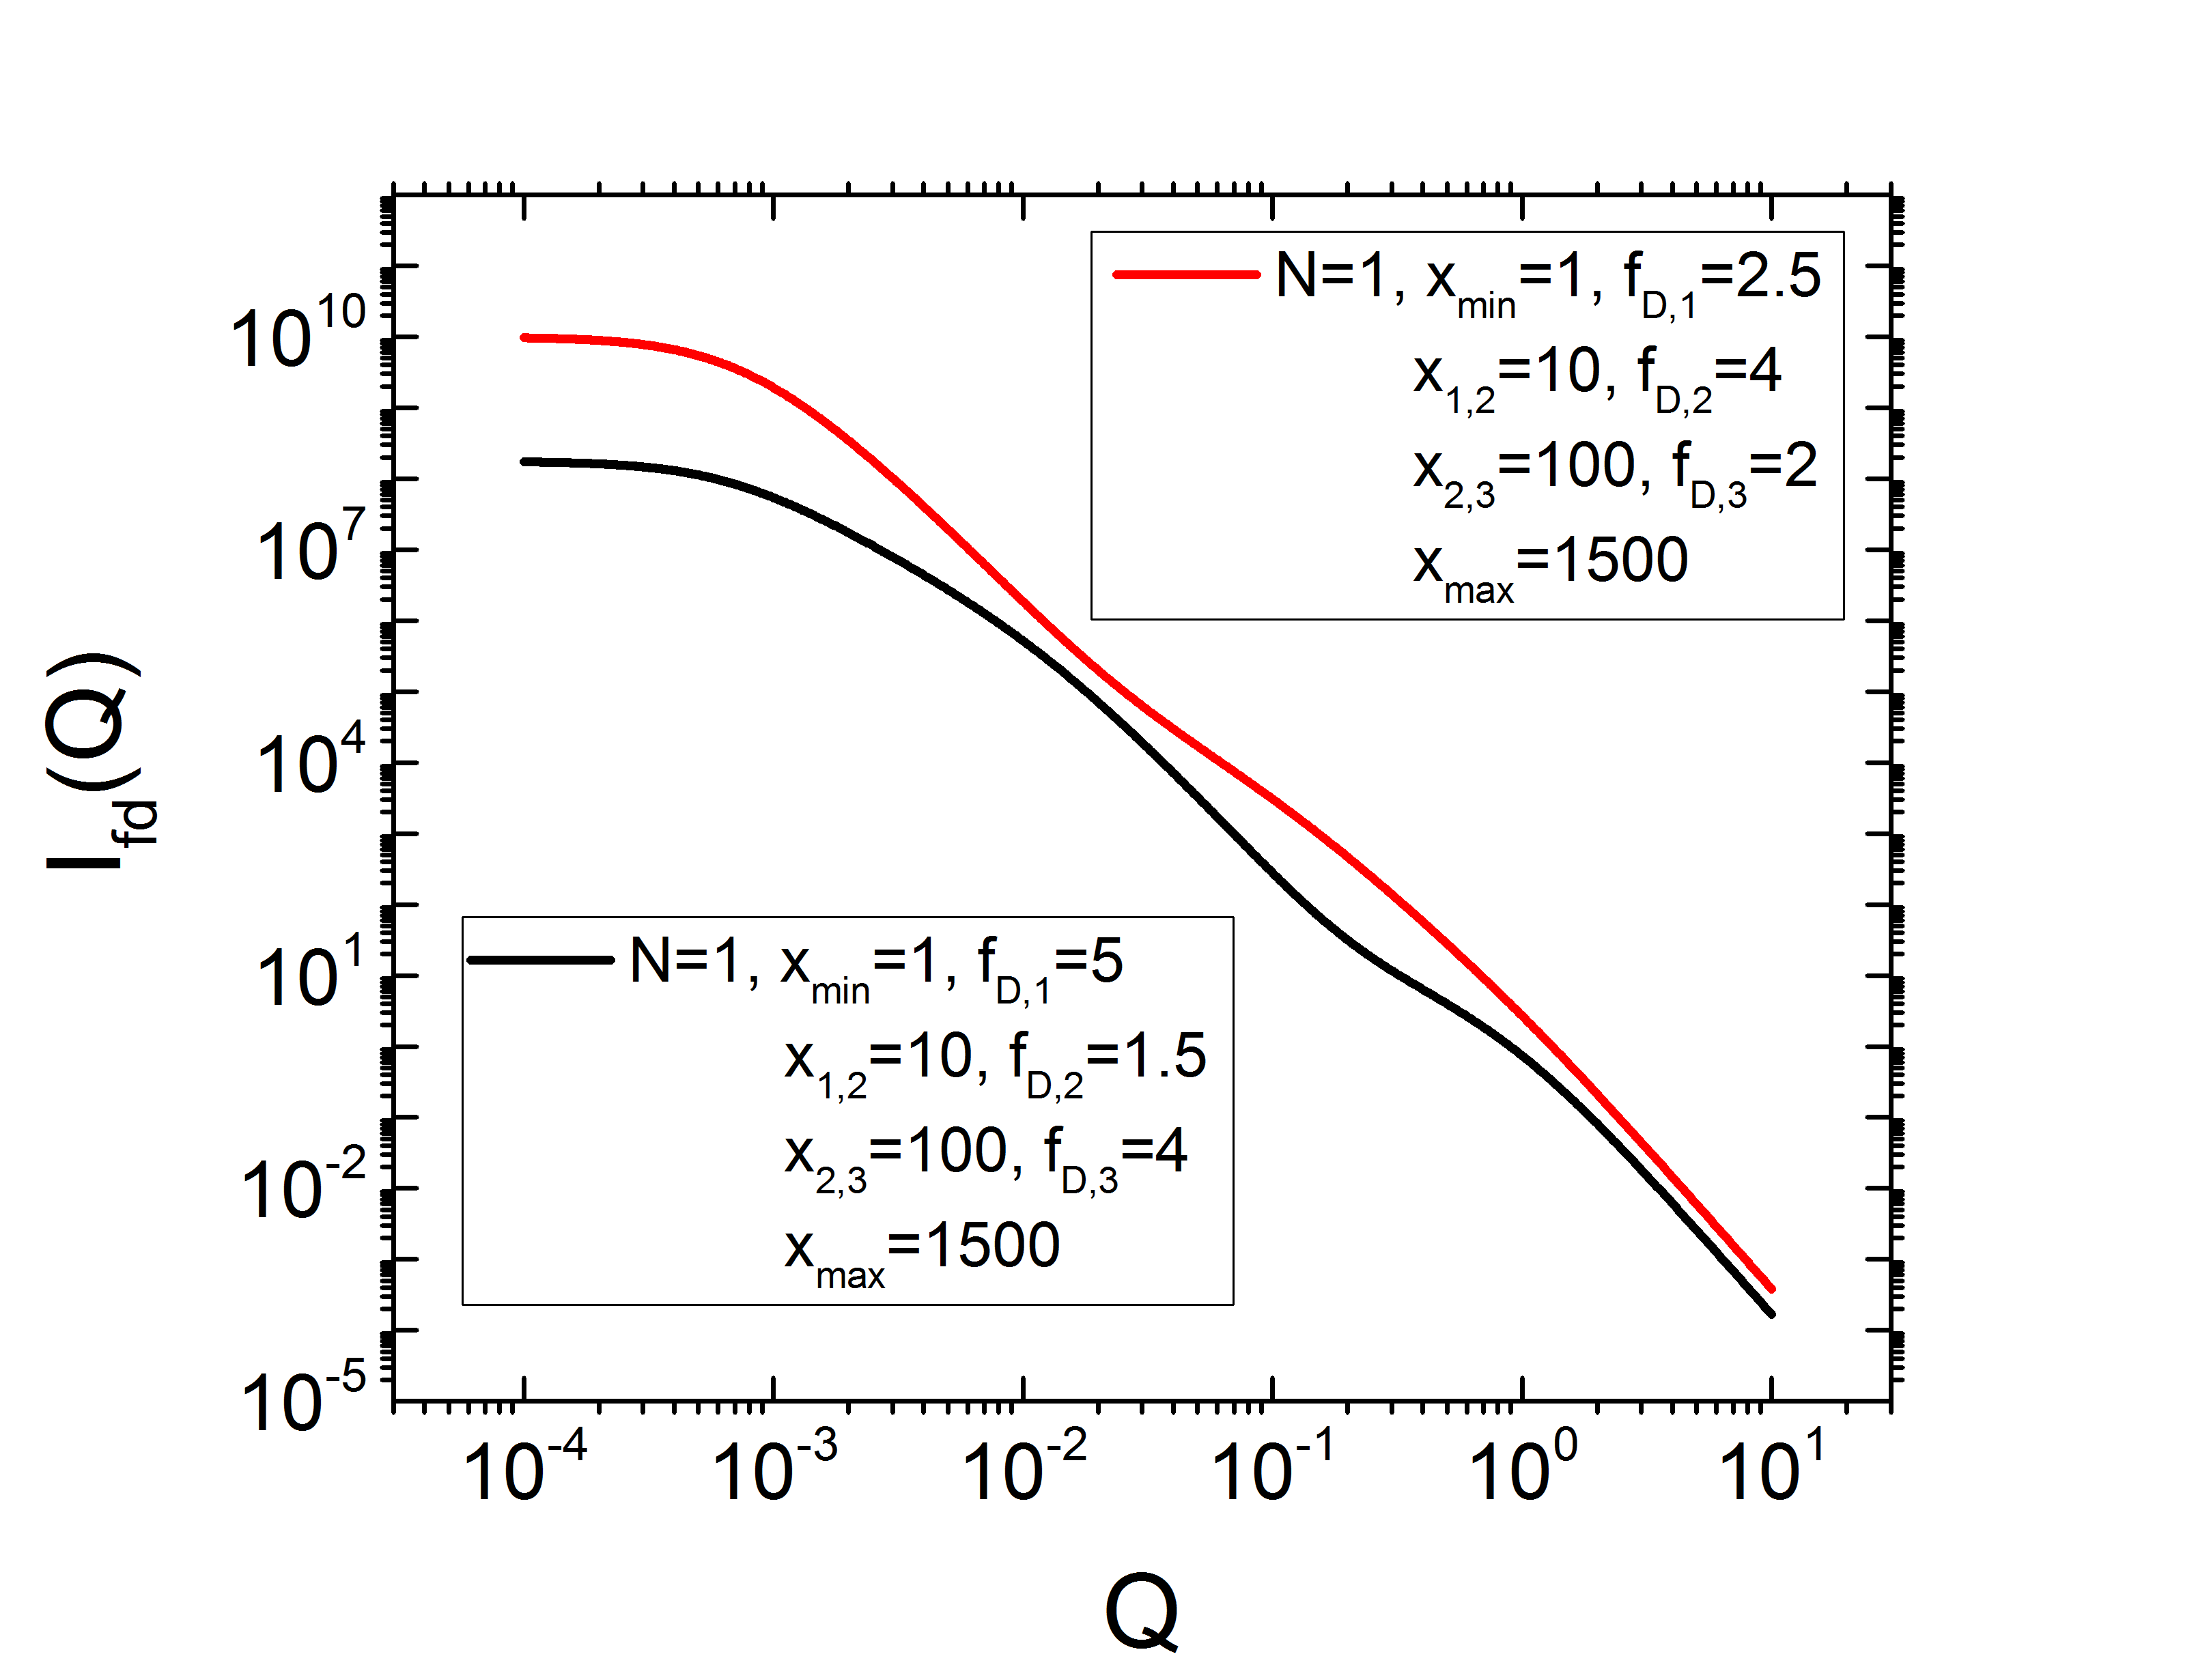
\includegraphics[width=0.47\textwidth]{../images/form_factor/fractal_series/fractalseries3IQ.png}}
\hfill
\subcaptionbox{fractal size distribution, the size distribution is zero for $x<x_\mathrm{min}$ and $x>x_\mathrm{max}$ \label{fig:fractalseries2} }{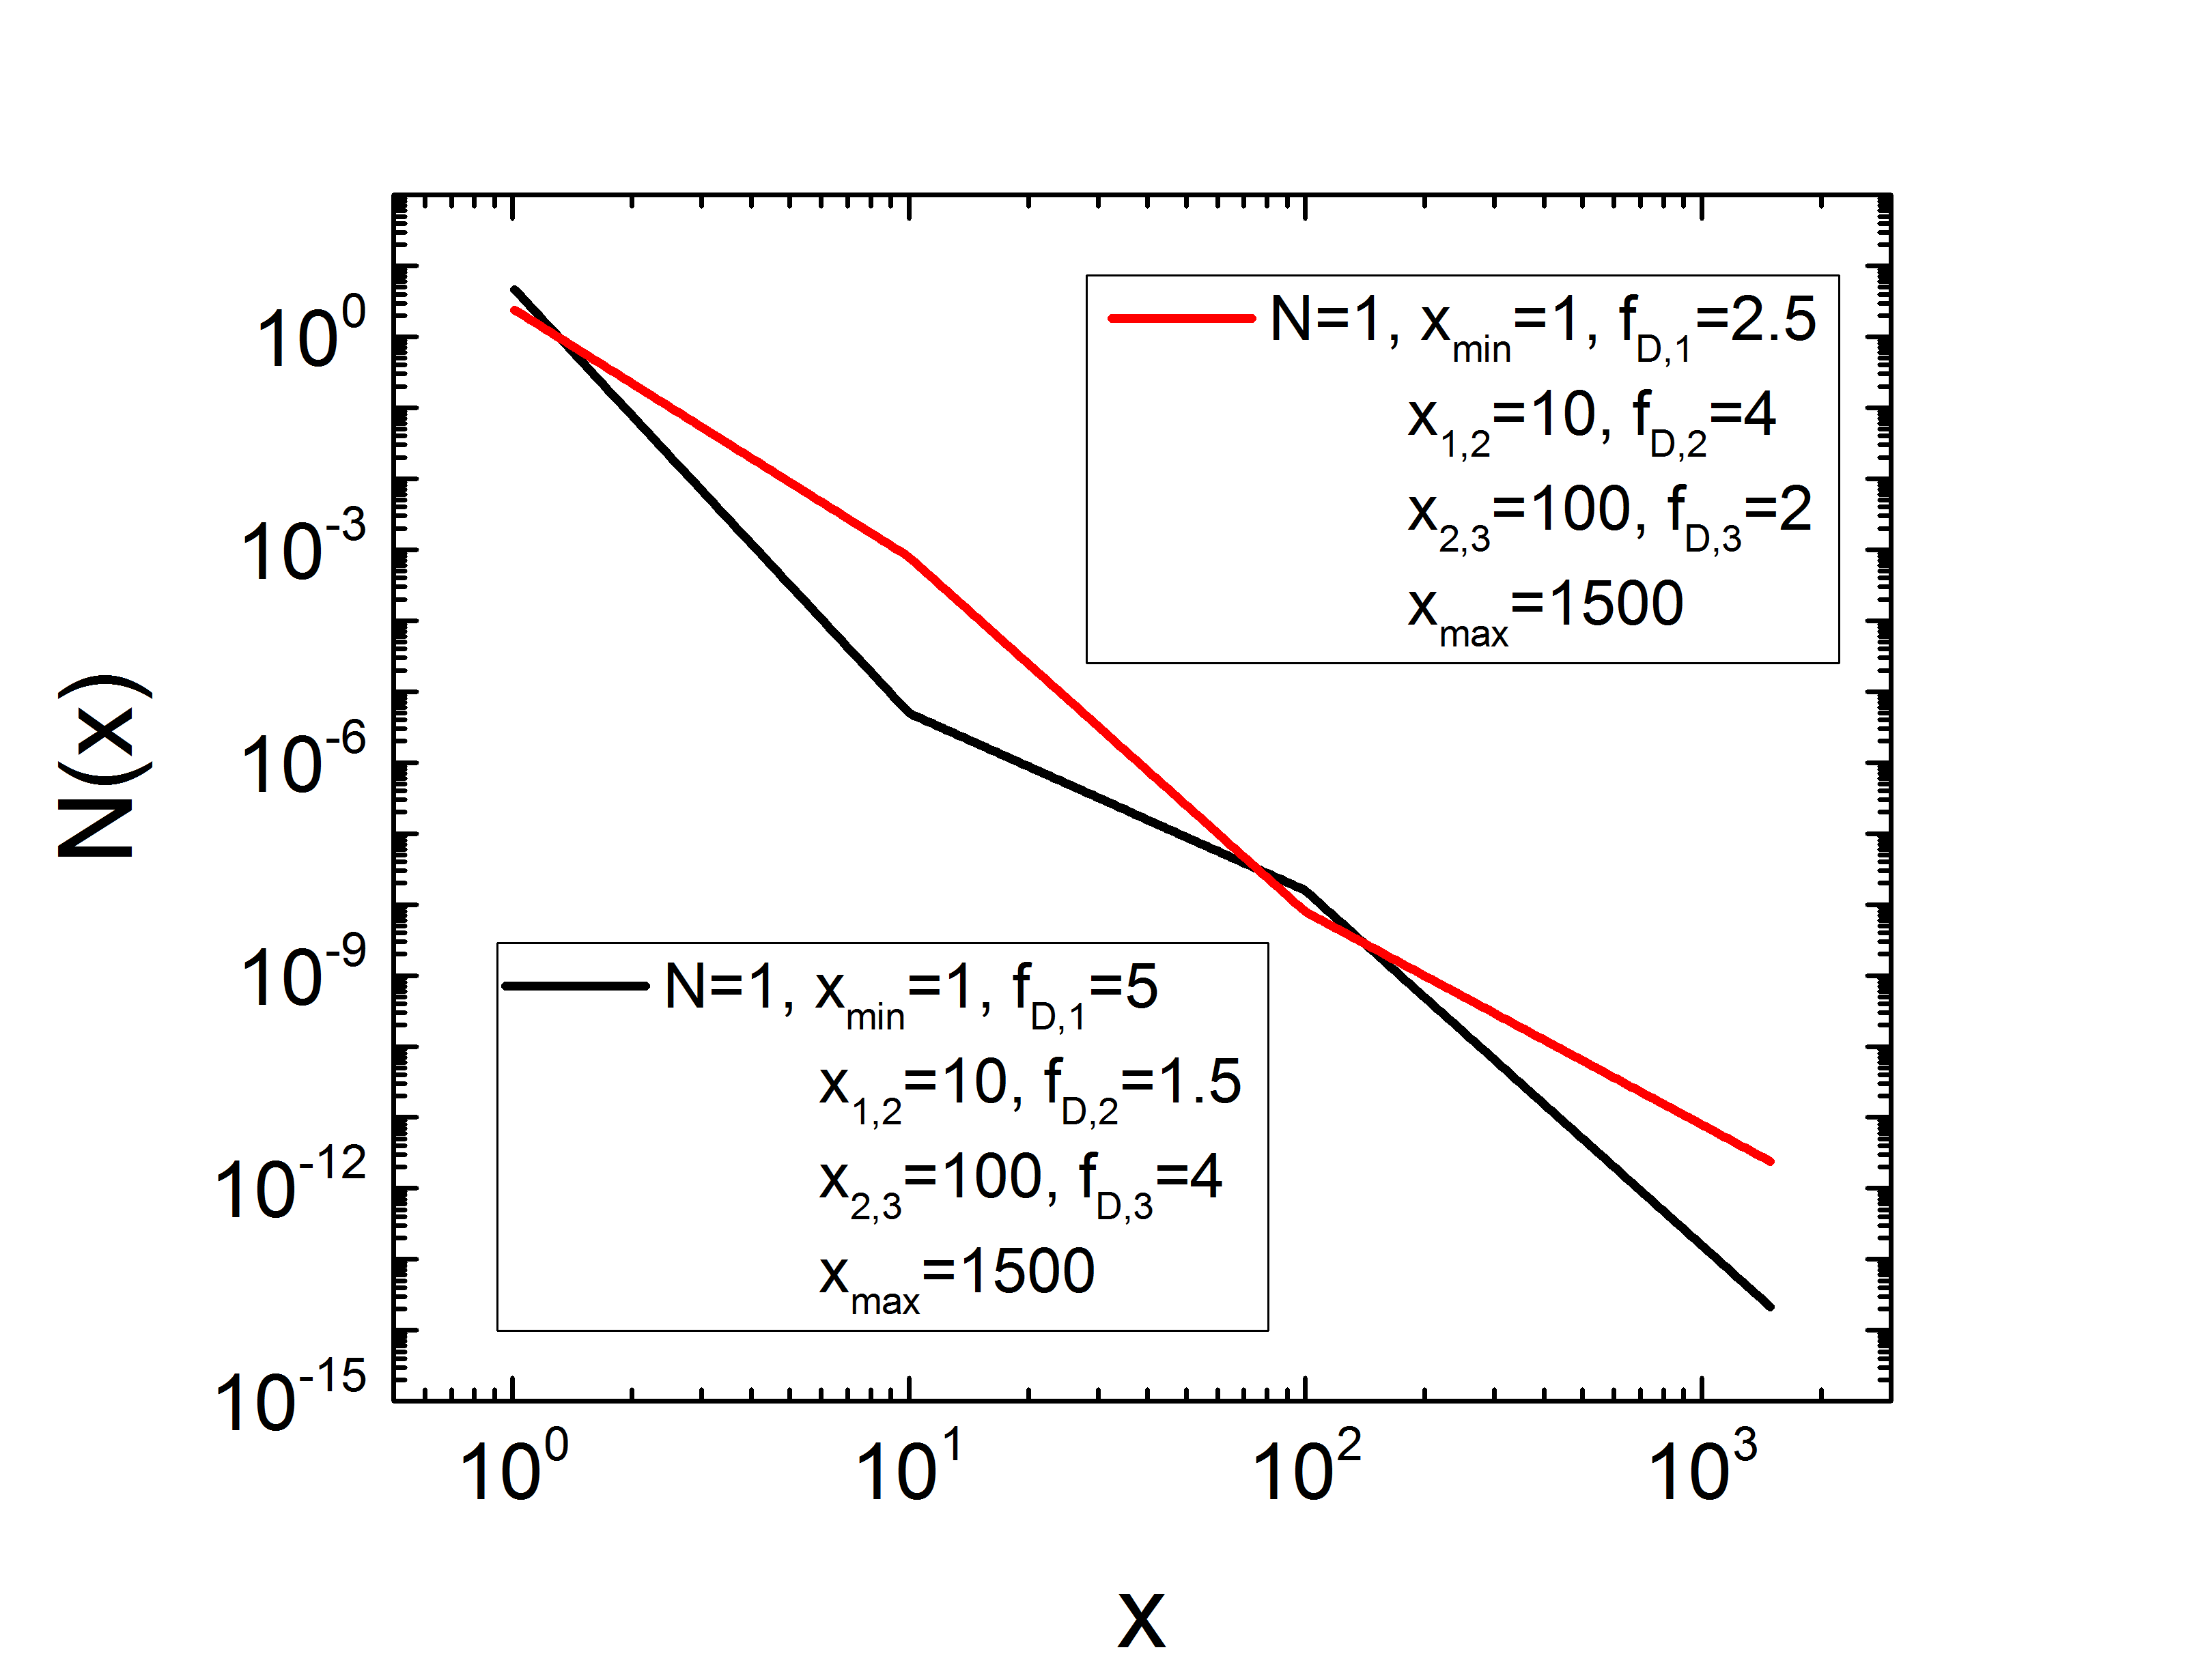
\includegraphics[width=0.47\textwidth]{../images/form_factor/fractal_series/fractalseries3Nx.png}}
\caption{Scattering curve and corresponding size distribution for the plugin "\texttt{fractal series 3}".}
\end{figure}

